%----------------------------------------------------------------------------------------

% Define some commands to keep the formatting separated from the content 
\newcommand{\keyword}[1]{\textbf{#1}}
\newcommand{\tabhead}[1]{\textbf{#1}}
\newcommand{\code}[1]{\texttt{#1}}
\newcommand{\file}[1]{\texttt{\bfseries#1}}
\newcommand{\option}[1]{\texttt{\itshape#1}}
\newcommand{\grados}{$^{\circ}$}

%----------------------------------------------------------------------------------------
%\section{Introducción}
%----------------------------------------------------------------------------------------

% Chapter 1

\chapter{Introducción} % Main chapter title
\label{Chapter1} % For referencing the chapter elsewhere, use \ref{Chapter1} 
\label{Intro}

Los sistemas de información visual suelen estar presentes en diversas industrias y aplicaciones. A grandes rasgos se componen de un sistema que genera o procesa información, una red de transmisión y finalmente carteles que exponen mensajes para que las personas los puedan consumir visualmente.\\

 Estos sistemas tienen un rol fundamental en la industria del transporte. Las personas se trasladan tanto por tierra como por aire usando distintos medios de transporte tales como automóviles, trenes o aviones. En cada uno de estos casos existen sistemas de información visual con diferentes características. En una autopista se suelen utilizar estos sistemas para comunicar eventos que suceden en algún tramo del recorrido a los conductores, como un choque o una obra vial en ejecución. En los trenes y aeropuertos estos sistemas tienen que estar sincronizados con el estado de la trayectoria del vehículo en cuestión. Los pasajeros en los aeropuertos consumen información del estado de los vuelos programados, en arribo o próximos a despegar. Los pasajeros en trenes usan estos sistemas para conocer la estación destino o la próxima estación cuando están viajando en una formación. \\

En este trabajo en particular se desarrolla el sistema de control para carteles de matriz led del sistema de información visual para pasajeros de trenes argentinos. Las formaciones de trenes argentinos cuentan con carteles de matriz led en los coches y en el frente y contrafrente del tren. Todos los carteles se interconectan a una red de comunicación transversal al tren. Por la misma red viajan datos que tienen distinto origen, como la información de sensores o los eventos que indican que un tren ha llegado a destino, por citar ejemplos. \\

Los carteles led van presentando fallas a lo largo del tiempo, motivo por el cual el personal de trenes tiene que realizar tareas de mantenimiento, reparación o reposición. Si bien existen muchos tipos de carteles led disponibles comercialmente, la integración al sistema de comunicación del tren es propietaria del fabricante de trenes. El desarrollo de un sistema a medida de los trenes es el eje de este trabajo. La necesidad que prima es generar y brindar al personal de trenes, asi como a los usuarios, de la información necesaria para construir estos sistemas de información visual.\\


En el capítulo 1 se introduce al lector a la motivación original del trabajo realizado. Se explica el marco de investigación del que forma parte este proyecto, se presenta el estado del arte en controles de carteles led.\\

En el capítulo 2 se introduce vocabulario técnico específico. Se presenta una descripción del sistema con el foco en la red de comunicaciones, el subsistema de visualización de información al pasajero, sus interacciones y componentes.\\

En el capítulo 3 se abordan cuestiones de diseño de sistema. Se especifican los requerimientos y casos de uso que se plantean en el espacio problema. Se detalla también la solución planteada en términos de arquitectura, patrones de software implementados, descripción de componentes e interfaces. Se incluye también circuitos eléctricos de las placas de hardware existentes al realizar este trabajo.\\

En el capítulo 4 se abordarán cuestiones relacionadas al entorno real del sistema: visitas técnicas, mediciones realizadas, hardware ad-hoc realizado para las mediciones y un breve análisis de las tramas de datos de la red PIDS existente.\\

En el capítulo 5 se tratan las conclusiones principales del desarrollo, su potencial fabricación en serie y los pasos a seguir para integrar al resto de ramales ferroviarios. En el apéndice de bibliografía se encontrarán las principales referencias técnicas, científicas e institucionales relevantes para este trabajo.\\


\pagebreak
\section{Introducción general}

El  marco de este trabajo es un Proyecto de Desarrollo Estratégico (PDE) de la Secretaría de Ciencia y Técnica de la Universidad de Buenos Aires (UBACyT). El PDE se titula PDE\_15\_2020 - "Sistema de monitoreo y gestión de la red TCN en formaciones ferroviarias". Las partes que se involucran y forman parte del equipo de trabajo en este proyecto son el Grupo de Investigación en Calidad y Seguridad de las Aplicaciones Ferroviarias (GICSAFE), creado en 2017 en el marco del Consejo Nacional de Investigaciones Científicas y Técnicas (CONICET) de la República Argentina, y la  Operadora Ferroviaria Sociedad del Estado (SOFSE), también conocida como Trenes Argentinos Operaciones. El proyecto está orientado a cubrir necesidades tecnológicas concretas del sistema ferroviario argentino. Este tipo de proyectos son instrumentos de promoción científico-tecnológica que revalorizan e incrementan el aporte de la Universidad al desarrollo socioproductivo.\\

El objetivo principal de este trabajo es diseñar e implementar un sistema de información visual para pasajeros a bordo del tren. El sistema de información visual para pasajeros existente tiene una parte manual y una automática. Cuando el conductor del tren toma cabina para brindar servicio, programa en una pantalla cuáles van a ser las estaciones cabecera. Los nombres de estas estaciones cabecera se visualizan en las marquesinas del frente y contrafrente del tren, como puede verse en la figura \ref{fig:tren}.

\begin{figure}[ht]
	\centering
	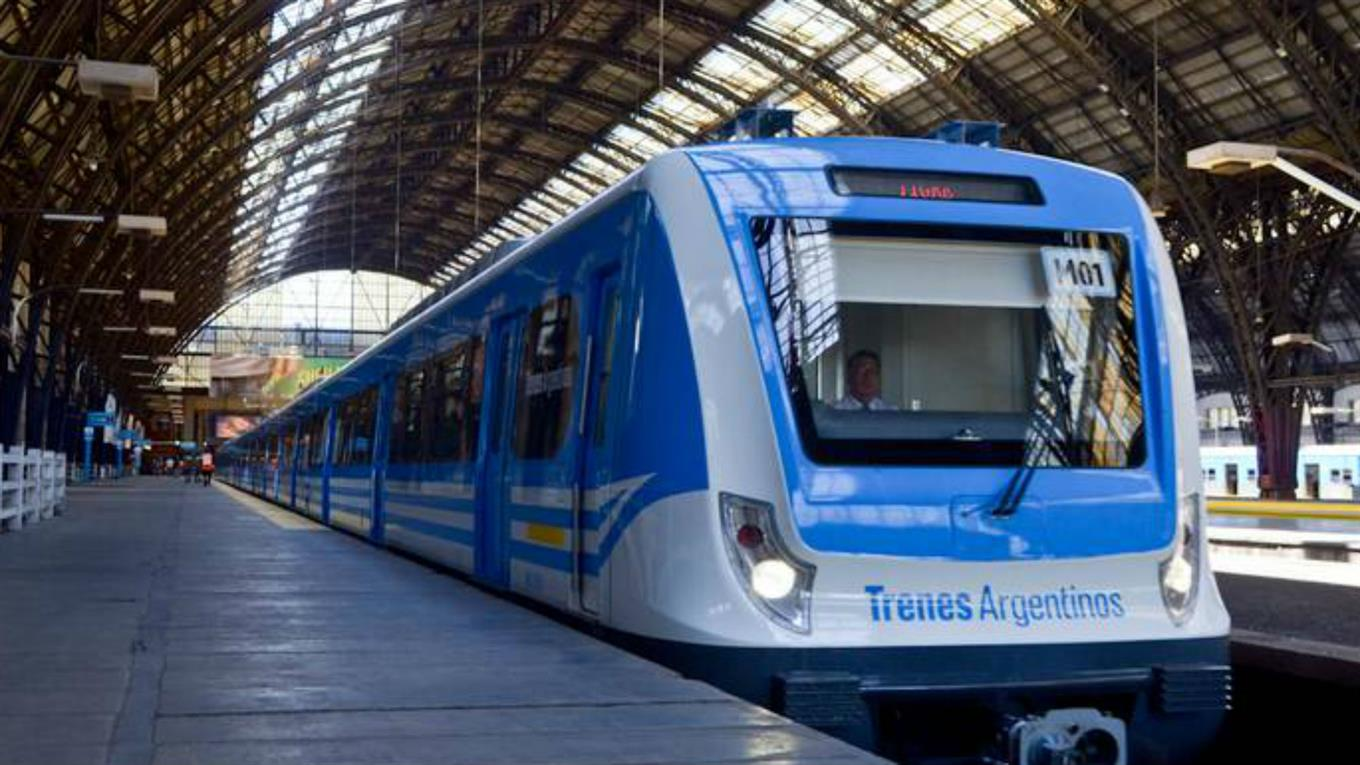
\includegraphics[width=1\textwidth]{./Figures/tren.jpg}
	\caption{Foto de una formación operativa de Trenes Argentinos. Se observa el cartel de matriz led frontal que indica el destino Tigre.}
	\label{fig:tren}
\end{figure}

\pagebreak
\section{Objetivos y alcance}

En el interior de los coches también hay marquesinas led. En estas marquesinas se presentan
mensajes a los pasajeros como el nombre de la próxima estación, o la estación arribada
(“próxima estación Belgrano”, “estás en estación Belgrano”, por ejemplo). Ésta información se
presenta automáticamente en base a variables de sistema que monitorean el detenimiento del
tren, su velocidad y la apertura o cierre de puertas. Esta y otra información de monitoreo y

control viaja por una red de comunicación interna del tren que se denomina TCN (Train
Communication Network) de acuerdo al estándar que la define [IEC-61375]. Este estándar define
para la red TCN dos buses jerárquicos donde se conectan los subsistemas electrónicos: el WTB
(Wire Train Bus) [3] y el MVB (Multi-Vehicle Bus) [4]. El primero es el bus de mayor jerarquía que
se conecta entre vagones y que se usa para monitorear cambios topográficos del tren. El
segundo se conectan los sensores y actuadores de cada coche como son los frenos, los
controles de puertas, los monitores de velocidad, el sistema de información, etcétera.
El sistema propuesto pretende leer del bus MVB los mensajes de información al pasajero que
viajan por la red TCN existente y presentarlos en un display LED. El sistema se compone
principalmente de cuatro partes:
● un display LED
● una placa de control y comunicación
● cables de interconexión
● firmware asociado
El diagrama del prototipo se presenta en la figura 2. El display LED matricial representa la
marquesina del tren. La placa de control se debe poder conectar al bus MVB de la red TCN
como entrada y al display LED como salida.


La placa de control estará basada en alguna de las plataformas desarrolladas por el
CONICET-GICSAFe. La conexión entre el display y la placa así como de la placa con la red TCN
deberá ser compatible con el estándar RS-485, definido como capa física en la red TCN. El
firmware a desarrollar se cargará a la placa de control usando el puerto USB de una laptop. Este
firmware será el responsable de leer los mensajes del sistema de información al pasajero y
presentarlos en el display.


Las necesidades que debe satisfacer este proyecto son:
● compatibilidad tecnológica: debe cumplir con los estándares asociados a la red TCN
● practicidad: debe ser de uso simple para el personal de Trenes Argentinos Operaciones
Este proyecto permitirá implementar las funciones de visualización del sistema de información al
pasajero sin depender del equipamiento existente. El sistema existente es un equipamiento
integrado y propietario, y este proyecto busca desacoplar algunas de las funciones, las que
corresponden a la visualización de información, y presentarlas en un display LED genérico. Por
otro lado, permitirá reponer los carteles que en la actualidad quedan fuera de servicio por fallas o
pérdida del material original y no pueden ser reparados. De esta manera, el valor principal que
aporta este proyecto es contribuir con la sustitución de repuestos faltantes por medio de
desarrollo y reducir la dependencia tecnológica de la empresa con los fabricantes. Este proyecto
tiene impacto directo en las formaciones ferroviarias existentes que brindan servicio al pasajero
todos los días.


En el trabajo se propone explorar los datos del sistema de información al pasajero que viajan por
la red TCN. Mediante la implementación de firmware sobre una placa de control se pretende
interpretar estos datos de sistema y presentarlos en un display LED. Algunos aspectos a resolver
incluyen:
● obtener datos del bus MVB asociados al sistema de información al pasajero
● controlar un display LED para presentar la información recibida del bus MVB
Para resolver estos aspectos se considera el desarrollo de firmware sobre un microcontrolador
con arquitectura de 32 bits. Usando la metodología del SWEBOK [6] se pretende garantizar
calidad de software. Con este enfoque se pretende generar documentación sistemática, simple y
de fácil lectura. La integración con la red TCN involucra el estudio de protocolos que usa la
comunicación del bus MVB, que se vinculan con la materia de Protocolos de Comunicación del
segundo bimestre. También existe la opción de usar sistemas operativos de tiempo real en la
placa controladora para obtener los mensajes a visualizar. Estos puntos se vinculan con las
materias del segundo y tercer bimestre de Sistemas Operativos de Tiempo Real. Las pruebas del
sistema se diseñarán en conjunto con las piezas de código funcional y de test en cada etapa.

\pagebreak
\section{Estado del arte}
El uso de carteles de matriz led es de uso muy extendido en distintas aplicaciones. Además de los trenes,  existen sistemas de información visual al pasajero en aeropuertos, en paradas de ómnibus, en señalamiento vial, en la industria del entretenimiento por mencionar algunos ejemplos. Las dimensiones del cartel, la densidad de píxeles por unidad de área, la cantidad de colores o leds por píxel, los niveles de intensidad lumínica, el brillo y contraste, la potencia eléctrica, son algunas de las especificaciones típicas.\\

 Los controladores de los carteles de matriz led suelen basarse en circuitos digitales, en microcontroladores de 8, 16 o 32 bits o en FPGA. La transmisión de datos y el formato de los mismos dependen de la implementación de cada sistema.  \\

En \cite{b1} se utiliza el chip AT89C52 para enviar caracteres chinos sobre matrices de 32 x 192 leds de un solo color; en \cite{b2} se implementa una pantalla led RGB de 320 x 240 píxeles que rota 360º permitiendo visualizar imágenes en color por persistencia de visión; en \cite{b3} se desarrollan algoritmos sobre FPGA usando búferes de datos para controlar una pantalla LED de 160 x 32 píxeles alcanzando 32,768 colores; en \cite{b4} se presenta el control de un micro display de transistores de película delgada (TFT) usando modulación por ancho de pulso (PWM) alcanzando 256 niveles de color a una frecuencia de refresco de 60 Hz, basado también en FPGA; en \cite{b5} se presenta el control de píxeles virtuales para matrices led multicolor usando flip-flops tipo D. \\

En el diseño e implementación del presente trabajo, los carteles son de matriz led de un solo color y de distintas dimensiones (8x64, 32 x 64, 32 x 128). El control de los carteles tiene como factor común el uso del conjunto de chips digitales 74HC138, 74HC595 y 74HC245. La topología permite interconectar paneles en serie para construir carteles led de distinto tamaño usando la misma lógica de control. \\

\pagebreak
\section{Bibliografía}
\label{sec:biblio}

Las opciones de formato de la bibliografía se controlan a través del paquete de latex \option{biblatex} que se incluye en la memoria en el archivo memoria.tex.  Estas opciones determinan cómo se generan las citas bibliográficas en el cuerpo del documento y cómo se genera la bibliografía al final de la memoria.

En el preámbulo se puede encontrar el código que incluye el paquete biblatex, que no requiere ninguna modificación del usuario de la plantilla, y que contiene las siguientes opciones:

\begin{lstlisting}
\usepackage[backend=bibtex,
	natbib=true, 
	style=numeric, 
	sorting=none]
{biblatex}
\end{lstlisting}

En el archivo \file{reference.bib} se encuentran las referencias bibliográficas que se pueden citar en el documento.  Para incorporar una nueva cita al documento lo primero es agregarla en este archivo con todos los campos necesario.  Todas las entradas bibliográficas comienzan con $@$ y una palabra que define el formato de la entrada.  Para cada formato existen campos obligatorios que deben completarse. No importa el orden en que las entradas estén definidas en el archivo .bib.  Tampoco es importante el orden en que estén definidos los campos de una entrada bibliográfica. A continuación se muestran algunos ejemplos:

\begin{lstlisting}
@ARTICLE{ARTICLE:1,
    AUTHOR="John Doe",
    TITLE="Title",
    JOURNAL="Journal",
    YEAR="2017",
}
\end{lstlisting}


\begin{lstlisting}
@BOOK{BOOK:1,
    AUTHOR="John Doe",
    TITLE="The Book without Title",
    PUBLISHER="Dummy Publisher",
    YEAR="2100",
}
\end{lstlisting}


\begin{lstlisting}
@INBOOK{BOOK:2,
    AUTHOR="John Doe",
    TITLE="The Book without Title",
    PUBLISHER="Dummy Publisher",
    YEAR="2100",
    PAGES="100-200",
}
\end{lstlisting}


\begin{lstlisting}
@MISC{WEBSITE:1,
    HOWPUBLISHED = "\url{http://example.com}",
    AUTHOR = "Intel",
    TITLE = "Example Website",
    MONTH = "12",
    YEAR = "1988",
    URLDATE = {2012-11-26}
}
\end{lstlisting}

Se debe notar que los nombres \emph{ARTICLE:1}, \emph{BOOK:1}, \emph{BOOK:2} y \emph{WEBSITE:1} son nombres de fantasía que le sirve al autor del documento para identificar la entrada. En este sentido, se podrían reemplazar por cualquier otro nombre.  Tampoco es necesario poner : seguido de un número, en los ejemplos sólo se incluye como un posible estilo para identificar las entradas.

La entradas se citan en el documento con el comando: 

\begin{verbatim}
\citep{nombre_de_la_entrada}
\end{verbatim}

Y cuando se usan, se muestran así: \citep{ARTICLE:1}, \citep{BOOK:1}, \citep{BOOK:2}, \citep{WEBSITE:1}.  Notar cómo se conforma la sección Bibliografía al final del documento. 
